\section{Gravitational Waves}

On February 11, 2016, the LIGO Scientific Collaboration announced the
first detection of gravitational waves from a black hole binary
inspirals, occurring on September 14, 2015, with pre-merger masses of
36 $M_\odot$ and 29 $M_\odot$ and a post merger mass of 62 $M_\odot$
at a redshift of $z=0.09$~\cite{GW150914}. Two subsequent detections
followed, on December 26, 2015~\cite{GW151226} and on January 4,
2017~\cite{GW170104}, with masses that are about the same to within an order of magnitude.

There is a question of what is meant, observationally, by a black hole. Does it need to have a horizon? Does it need to have a Kerr metric (the simplest possible space-time for a spinning black hole in general relativity)? Does it simply need to be a sufficiently compact object that it can't be ordinary nuclear matter? Historically, black holes have been defined by their compactness~\cite{Bambi2017}; however, some studies are beginning to consider tests of horizons~\cite{} or of the Kerr metric itself~\cite{Bambi2017}. X-ray binaries, gravitational wave constraints from binary-pulsar systems, active galactic nucleii models containing super-massive black holes on the order of $10^6 M_\odot$, and the three LIGO detections, as well as black hole formation models, suggest that black holes of all scales should be spinning~\cite{Bambi2017}. However, for the purposes of this manuscript, I will consider non-spinning, spherically symmetric black holes in general relativity, described by the Schwarzschild metric.

Currently, there are four distinct windows on the gravitational wave universe planned or in progress. The Laser Interferometer Gravitational Wave Observatory, LIGO, probably deserves first listing, due to their recent success. LIGO observes gravitational waves using a ground based Michelson-Morley interferometer with two 4 kilometer long Fabry-Perot cavity arms. It detects strains as small as $10^{-23} Hz^{-1/2}$~\cite{LIGOsensitivity}. It has thusfar had three detections of blackhole binary pairs in the tens of solar mass range. These mergers have been tracked through inspiral and merger~\cite{GW150914}~\cite{GW151226}~\cite{GW170104}, and ringdown~\cite{LIGO1e}, to produce exact tests of general relativity. LIGO has even been able to set limits on non-General Relativistic behavior, such as the magnitude of the dispersion of the intergalactic medium to gravitational waves~\cite{GW170104} and deviation of the post Newtonian parameters from those predicted from GR~\cite{LIGO1e}. The LIGO-Virgo collaboration continues searches for neutron star binary inspirals, which may have electromagnetic counterparts in the form of supernovae; pulsars, which are thought to have raised ``mountains'' their surface causing a changing quadrupole moment-- these will also have electromagnetic counterparts; gravitational wave bursts correlated with EM, neutrino, or particle sources such as a gamma ray burst; or the cosmic or galactic white dwarf binary stochastic background radiation. In the future, KAGRA, an observatory in Japan, and IndIGO, an observatory in India, will join the search for gravitational waves, refining the collaboration's ability to locate a source on the sky. Geo600 is an existing English gravitational wave detector in England. The Einstein Telescope is a next generation gravitational wave detector that has also been proposed. 


The cosmic microwave background (CMB) can also be used to constrain the primordial stochastic baground of graviational waves. It is a very low frequency source, with wavelengths related to the size of the observable universe ($f\sim 10^{-17} Hz$). Searches depend upon separating the polarization into two components: the B-modes, which have curl, and the E-modes, which don't. If the B-modes and the E-modes are roughly even, then tensor components of the density perturbation dominate, and gravitational waves may be present. Microlensing and dust are significant noise sources that must be carefully subtracted. Current searches include BICEP2, Planck, and the Keck Array. Planned ground and balloon borne expreiments include the ACTPol, Polarbear, CLASS, Piper, and Spider. Planned space-base experiments include COrE, PRISM, LiteBIRD, and PIXIE~\cite{bmodes}. 


Pulsar timing uses the extremely precise timing of pulsars, taking their spin down into account and correlating with pairs of other pulsars. In this timing, they are looking for residual signals that may be due to supermassive black hole binaries, cosmic string cusps, and the cosmic stochastic gravitational wave background. Existing pulsar timing arrays include the Parkes Pulsar Timing Array (PPTA), the Eurpeoan Pulsar Timing Array (EPTA), and the North American Nanohertz Observatory for Gravitational Waves (NANOGrav). They have formed a collaboration called the Interanational Pulsar Timing Array (IPTA). The IPTA is sensitive from $10^{-9}$ to $5\times10^{-8}$ Hz with strains on the order of $10^{-14}$ to $10^{-15}$~\cite{hobbs_dai}.

Extreme mass ratio black hole binaries are likely to be detected only by LISA. The Laser Interferometer Space Observatory (LISA) is a space-based observatory

Intermediate mass blackhole binary systems are hypothesized to exist based on supermassive blackhole formation scenarios, but there is no indirect evidence for their existence through electromagnetic observational strategies. 


%\begin{figure}
%  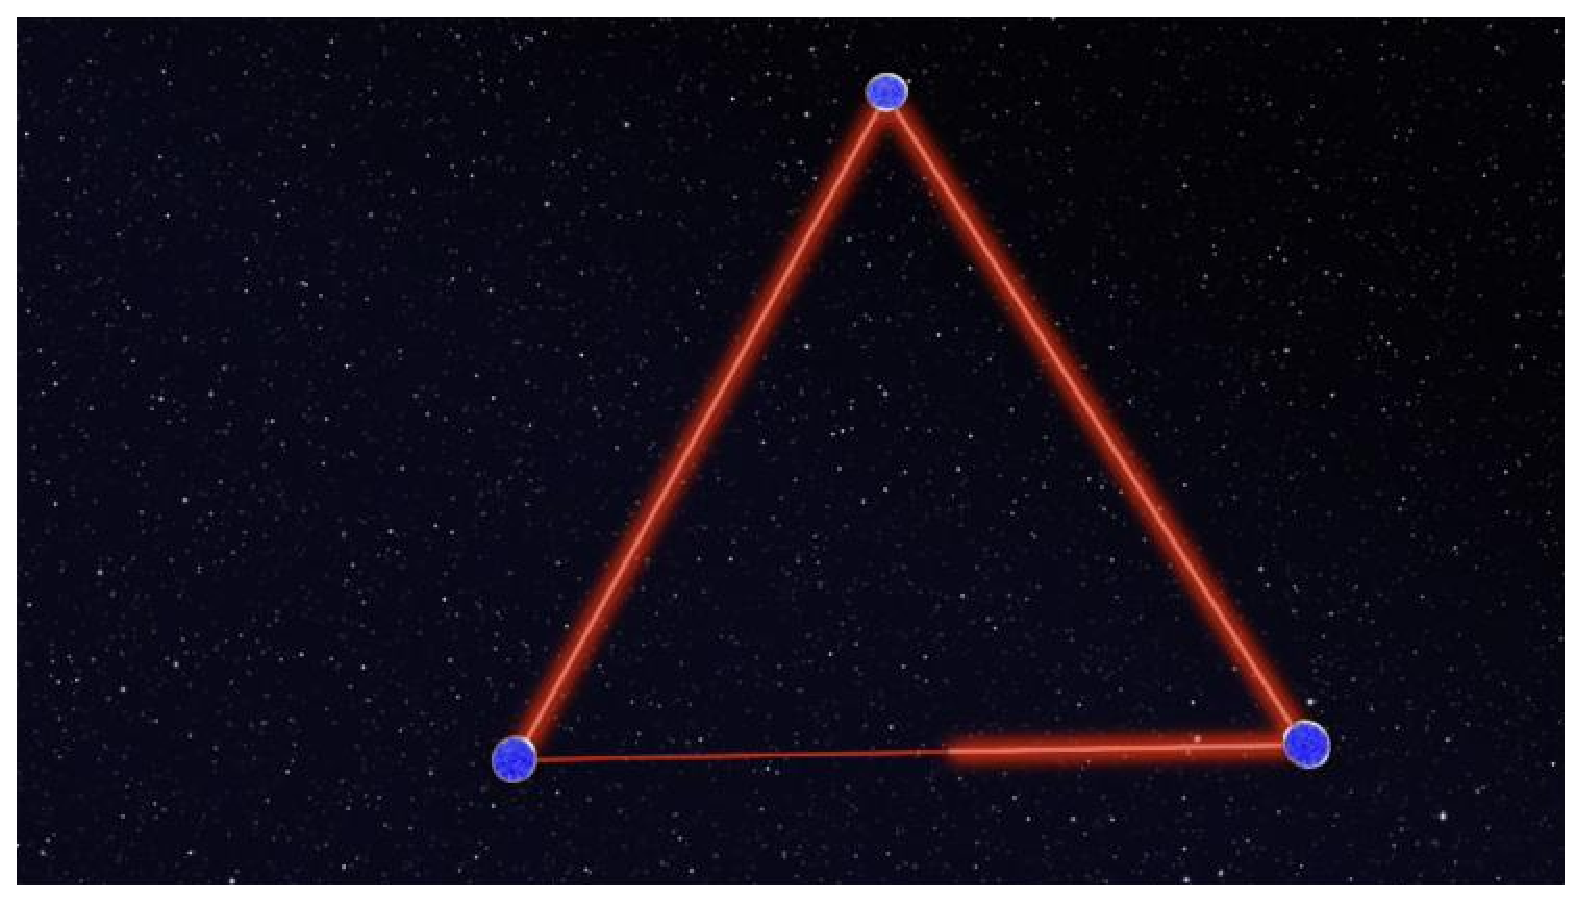
\includegraphics{eLISA}
%\end{figure}

%\begin{figure}
%  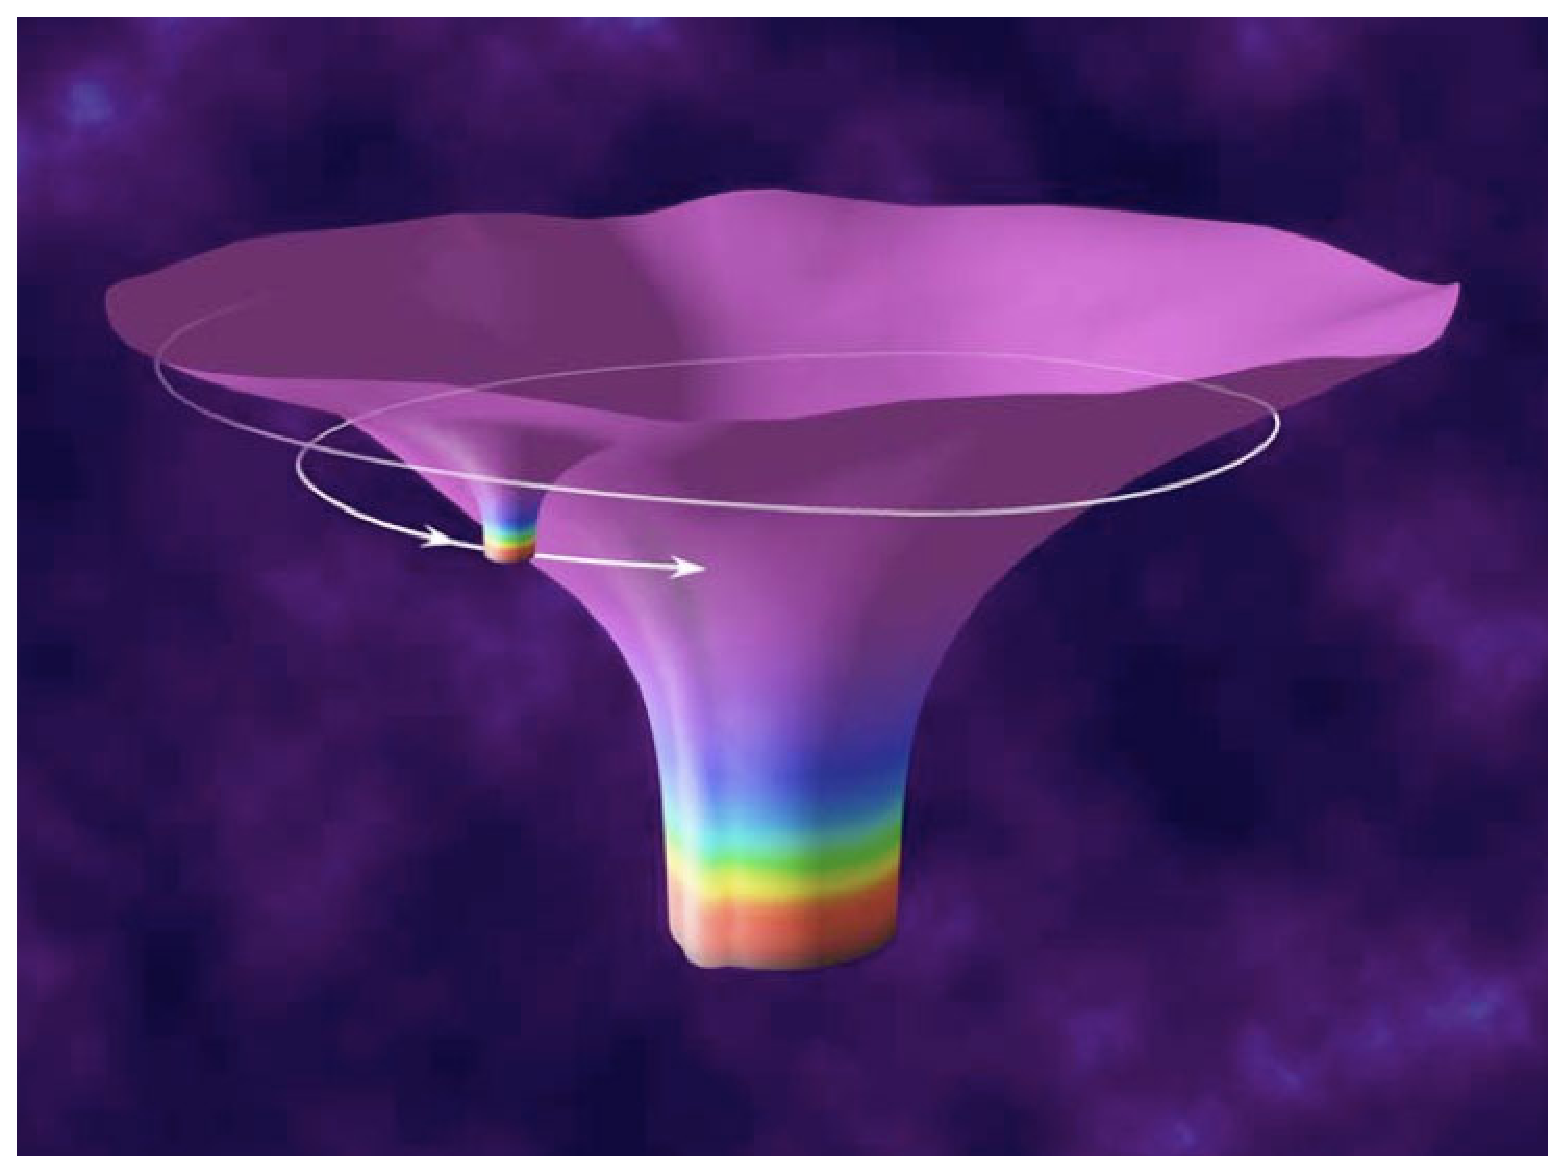
\includegraphics{EMRI}
%\end{figure}



%Thornberg
%Warburton
%Wardell
%Diener
%adam pound
%bernard whiting
%ian vega
%anna hesthaven
%maarten van de meent
%jonathan thompson
%jordan moxon?

\section{Extreme Mass Ratio Inspirals}
\section{LISA}
~\cite{LISA02062017}
~\cite{LISAscienceMarch28_2017}
~\cite{ELISAz}
~\cite{eLISAastrophysicsSelfForce}
\section{Self force}
EMfirst~\cite{dirac1938}
circular orbits, spherical harmonics, world tube~\cite{wardell_vega_thornberg_diener}
gravitational DG wave eq, elliptical~\cite{time_dependent_coordinate_transform}
2nd order self force~\cite{pound2ndOrderSelfForce0}
MiSaTaQuWa?~\cite{minosasakitanaka}
basis for code~\cite{heffernan_ottewil_wardell_modesum_basisForCode}



\section{Notation}
In this manuscript, I use Einstein summation notation for tensors, where a repeated Greek index implies a summation over that repeated index. For example, an $n$ dimensional tensor field of rank (1,2) transforms, in general, according to the rule
\begin{equation}
  T^\alpha_{\beta\gamma}(\bar{x}^1,\ldots,\bar{x}^n)=\Lambda^\alpha_\delta\Lambda^\epsilon_\beta\Lambda^\zeta_\gamma T^\delta_{\epsilon\zeta}(x^1,\ldots,x^n)
\end{equation}
where $\Lambda$ is the jacobian of the coordinate transformation from $x$ to $\bar{x}$. 

Indices are raised by use of the inverse metric and lowered by use of the metric. The metric transforms contravariant one-forms, which constitute the basis, to covariant vectors, which constitute the coordinates, e.g. $u^\beta=g^{\alpha\beta}u_\beta$, where $g^{\alpha\beta}$ is the metric. However, the metric and its inverse can also be used to raise and lower indices of tensors of higher and mixed rank. The metric describes the relative distance between two coordinates on a manifold, in all $n$ dimensions, in an $n\times n$ matrix. Two sign conventions are allowed, depending on whether the time component is positive or negative, though the metric always has a negative determinant in four dimensions. In our sign convention, the Minkowski metric for flat spacetime is given by
\[
\eta^{\mu\nu}=
\begin{bmatrix}
  -1 & 0 & 0 & 0\\
  0 & 1 & 0 & 0\\
  0 & 0 & 1 & 0\\
  0 & 0 & 0 & 1\\
\end{bmatrix}
\]
Here the four dimensions are Cartesian, $t$, $x$, $y$, and $z$. The Schwarzchild metric for a spherically symmetric blackhole without charge or spin is given by
\[
d\tau^2=g^{\mu\nu}
\begin{bmatrix}
  -(1-\frac{2M}{r}) & 0 & 0 & 0\\
  0 & (1-\frac{2M}{r})^{-1} & 0 &0\\
  0 & 0 & r^2 & 0\\
  0 & 0 & 0 & r^2\sin^2\theta
\end{bmatrix}
\]
where $d\tau$ is the proper time, and coordinates are $t$ (the local time), $r$ (a radial coordinate that goes to zero at the singularity, $2M$ at the horizon, and infinity at spatial infinity), $\theta$ (the polar angle), and $\phi$ (the azimuthal angle). To obtain the inverse (lowered) metric, simply invert the matrix representation.
